\subsection{Дифракция на решетке как краевая задача}

\subsubsection{Метод Рэлея}
Пусть решетка -- бесконечна, её переднюю поверхность будем называть \textbf{входом}, а заднюю -- \textbf{выходом}. Плоскость решетки примем за $XY$, а ось $Z$ по распространению волны.

Падающую волну представим в виде: $E_0 = A e^{i (\omega t - \smallvc{k} \smallvc{r})}$.
Тут полагаем $z = 0$, ищем поле на входе решетки, в силу линейности: 
\begin{equation*}
	E_{\text{вых}} = D E_{\text{вх}}.	
\end{equation*}	


Здесь введен коэффициент пропускания $D$ решетки. 
Теперь чтобы решить задачу о дифракции на решетки нам достаточно найти $D$, тогда мы уже будем знать поле на выходе из решетки, а значит и во всем пространстве дальше. Уравнение
\begin{equation*}
	\Delta E + k^2 E = 0
\end{equation*}
должно при $z = 0$ переходить в $E_{\text{вых}}(x,y) = D(x,y) E_{\text{вх}}(x,y)$. Такой подход к решению задача называется \textit{методом Рэлея}.

Для одномерной решетки можно представить $D$ как функцию с периодом $d$:
\begin{equation*}
	D = \sum_{m =- \infty}^{+\infty}D_m e^{-i m p x},
	\hspace{0.5 cm}
	p =\frac{2 \pi}{d}.
\end{equation*}
Таким образом:
\begin{equation*}
	E_\text{вых} = D E_\text{вх} = \sum_{m = - \infty}^{+\infty} A D_m e^{i [\omega t - (k_x + m p)x]}.
\end{equation*}
Общим решением нашего волнового уравнения будет:
\begin{equation*}
	E = \sum_{m = - \infty}^{+\infty} a_m e^{i(\omega t - \smallvc{q_m} \vc{r})},
\end{equation*}
на которое надо наложить в связи с граничным условием:
\begin{equation*}
	q_{mx} = k_x + m p, \hspace{0.5 cm} q_{m y} = 0.
\end{equation*}
И так как $\vc{q}^2 = k^2$, то $q_{mz} = \sqrt{k^2 - q_{mx}^2}$ -- для однородных волн и $q_{mz} = -i \sqrt{k^2 - q_{mx}^2}$ для неоднородных (поверхностных).

Тогда для поля на выходе можно написать:
\begin{equation*}
	E_\text{вых} = \sum_{-\infty}^{+\infty} a_m e^{i (\omega t - q_{mx} x)}
	\hspace{0.5 cm}
	\Rightarrow
	\hspace{0.5 cm}
	a_m = A D_m.
\end{equation*}

Теперь если $k_x = \left(\frac{2\pi}{\lambda}\right)\sin \theta$, $q_{mx} = \left(\frac{2\pi}{\lambda}\right) \sin\vartheta_m$ и $p = 2\pi/d$ то получаем основную формулу дифракционной решетки:
\begin{equation*}
	d (\sin \vartheta_m - \sin \theta) = m \lambda.
\end{equation*}
Что видим? Спектр за решеткой состоит из одних только главных максимумов, но это нормально, так как решетка бесконечна. 
В формулу для волны входят как однородные так и не однородные волны, а значит она описывает поле на любых расстояниях от решетки.
При нормальном падении света наивысший порядок однородных волн $m\leq d/\lambda$, иначе имеем неоднородные волны, которые затухают как $\exp(-\chi_m z)$, где
\begin{equation*}
	\chi_m = \sqrt{k^2 - q_{mz}^2} = \frac{2 \pi}{d} \sqrt{m^2 - (d/\lambda)^2}.
\end{equation*}

Интересно по-исследовать поле далеко от решетки. При $z \gg d$ оно состоит только из однородных волн. А если $d<\lambda$ то вообще из одной плоской волны ($m = 0$). 

Тут можно найти красивый эффект \textbf{саморепродукции}. 
Каждое слагаемое в разложении нашей волны -- поле плоской волны с пространственной частотой: $u_n = n \frac{2 \pi}{d}$. Для точки отстоящей на $z$ от решетки фаза $n$-ой плоской волны:
\begin{equation*}
	\varphi_n = \chi_n z = \sqrt{k^2 - q_{nx}^2} \approx k z - \frac{z q_{nx}^2}{2 k},
\end{equation*}
что верно для волн с узким спектром $|q|\ll k$.

Сравним набег фаз $n$-ой плоской волны с $\varphi_0 = kz$:
\begin{equation*}
	\Delta \varphi_n = \varphi_0 - \varphi_n = \frac{z}{2k}\left(\frac{2 \pi}{d}\right)^2 n^2 = \pi \frac{\lambda z}{d^2}n^2.
\end{equation*}
В плоскости наблюдения отстоящую от решетки на $z_1 = \frac{2 d^2}{\lambda}$ (это будет находится в зоне френелевской дифракции) будем иметь разность фаз $\Delta \varphi_n = 2 \pi n^2$. Заметим так же, что разность фаз от любых двух плоских волн будет $\Delta \varphi = 2 \pi (n_1^2 - n_2^2)$ тоже кратна $2\pi$. 
Значит в разложении волны ничего не меняется, так как это период, значит в плоскости $z_1$ поле повторяет по интенсивности пропускающую функцию решетки, ну а точнее:
\begin{equation*}
	f(x,z_1) = e^{i k z_1}f_0(x).
\end{equation*}
Это же свойство повторения характерно и для
\begin{equation*}
	z_m = m \frac{2 d^2}{\lambda} \, (m = 1,2 \ldots).
\end{equation*}
Этот эффект еще также носит названия \textbf{эффекта Таблота}.


Теперь посмотрим на небесконечную решетку.
\begin{equation*}
	D(x) = \int_{-\infty}^{+\infty} C(f) e^{-i f x} d f.
\end{equation*}
На выходе поле:
\begin{equation*}
	E_\text{вых} = A \int_{-\infty}^{+\infty} C(f) e^{-f(k_x +f)x}d f.
\end{equation*}
Решение тогда будет:
\begin{equation*}
	E = A \int_{-\infty}^{+\infty} C(f) e^{- i \smallvc{q} \smallvc{r}} d f.
\end{equation*}
Задавая функцию пропускания для такой конечной решетки:
\begin{equation*}
	D(x) =\left\{
	\begin{aligned}
		&0, &\text{ если } -\infty < x < - L,\\
		&\sum_{-\infty}^{_\infty} D_m e^{i m p x}, &\text{ если } - L < x < + L,\\
		&0, &\text{ если } + L < x < +\infty.\\
	\end{aligned}
	\right.
\end{equation*}
Вычислим коэффициент Фурье:
\begin{equation*}
	C(f) = \frac{1}{2 \pi} \int_{- \infty}^{+\infty} D(x) e^{i f x} dx = \frac{1}{\pi} \sum_{-\infty}^{+\infty} D_m \frac{\sin[L (f - mp)]}{f - mp}.
\end{equation*}
И получаем:
\begin{equation*}
	E = \sum_m E_m = \frac{A}{\pi} \int_{-\infty}^{+\infty} D_m \frac{\sin[L(f-mp)]}{f - mp}e^{-i \smallvc{q} \smallvc{r}} d f = \frac{A d}{\pi} \int_{-\infty}^{+\infty} D_m \frac{\sin[(N/a)(f d - 2 m \pi)]}{f d - 2m \pi}e^{i \smallvc{q} \smallvc{r}} d f.
\end{equation*}
Интенсивность такой волны достигает максимума когда знаменатель обращается в нуль, то есть когда $q_x = k_x + mp = 0$. Получаем направление на главный максимум:
\begin{equation*}
	\frac{\sin [(N/2)(fd - 2 m\pi)]}{(f d - 2 m \pi)} = \frac{N}{2}
\end{equation*}
Так же можно определить направления на главные минимумы. В итоге получили все очень зачетающимся с теорией про диф решетки и даже больше!

Стоит ещё сказать про \textbf{соотношение неопределенности}.

Рассматривая щель $b$ освещаемую нормально падающей волной имеем для выходной волны:
\begin{equation*}
	f_0(x) = \left\{
	1, \, |x| \leq b,\\
	0, \, |x| \geq b.
	\right.
\end{equation*}
Фурье коэффициент находим как:
\begin{equation*}
	C_0(u) = b \frac{\sin \frac{b}{2}u}{\frac{b}{2}u}
\end{equation*}
Тут ширина первого максимума составляет $|\Delta u|\lesssim \frac{2 \pi}{b}$
\begin{figure}[ht]
    \centering
    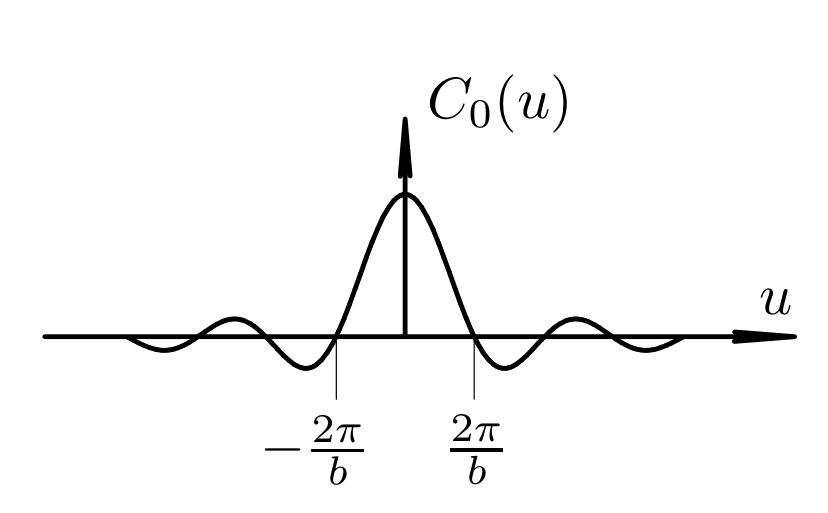
\includegraphics[width=0.3\textwidth]{figures/328.png}
    \caption{К соотношению неопределенностей на плоской щели.}
    %\label{fig:}
\end{figure}
Посмотрев на пропускание щели заметим соотношение неопределенности:
\begin{equation*}
	\Delta x \cdot \Delta u \sim 2 \pi.
\end{equation*}
Пространственная протяженность $\Delta x$ определяется характером самого препятствия. Разброс же плоских волн за отверстием даёт дифракционную расходимость пучка света за отверстием:
\begin{equation*}
	\Delta u = k \Delta(\sin \alpha)
	\hspace{0.5 cm}
	\Rightarrow
	\hspace{0.5 cm}
	\Delta(\sin \alpha) \approx \frac{\lambda}{b}
	\hspace{0.5 cm}
	\Rightarrow
	\hspace{0.5 cm}
	\Delta \alpha \approx \frac{\lambda}{b}.
\end{equation*}
% \subsubsection{Эффект Саморепродукции}
% Возьмём\footnote{тут всё взято из лабника потому буквенные обозначения могут отличаться от тех, что написаны в Сивухине.} экран с щелями ширины $b$ на расстоянии $d$ друг от друга. Осветим его нормально падающей волной $\lambda$. Взяв $D$ как единица на щели и ноль на штрихе:
% \begin{equation*}
% 	f_n = \sum c_n e^{i n \frac{2 \pi}{d} x}
% \end{equation*}
% Каждое слагаемое -- поле плоской волны с пространственной частотой: $u_n = n \frac{2 \pi}{d}$. Для точки отстоящей на $z$ от решетки, как было показано ранее:
% \begin{equation*}
% 	f(x,z) = \sum c_n e^{i (u_n x + \sqrt{k^2 - u_n^2}z)}
% \end{equation*}
